\section{Eindimensionale Richtungsbestimmung} \todo{Durchlesen + überprüfen}
  Um den Algorithmus, der aus den Phasendifferenzen den Ort zurückrechnet zu entwickeln haben wir mit der
einfachsten Stufe der Richtungsbestimmung, der eindimensionale Richtungsbestimmung, angefangen:
\begin{figure}
  \centering
  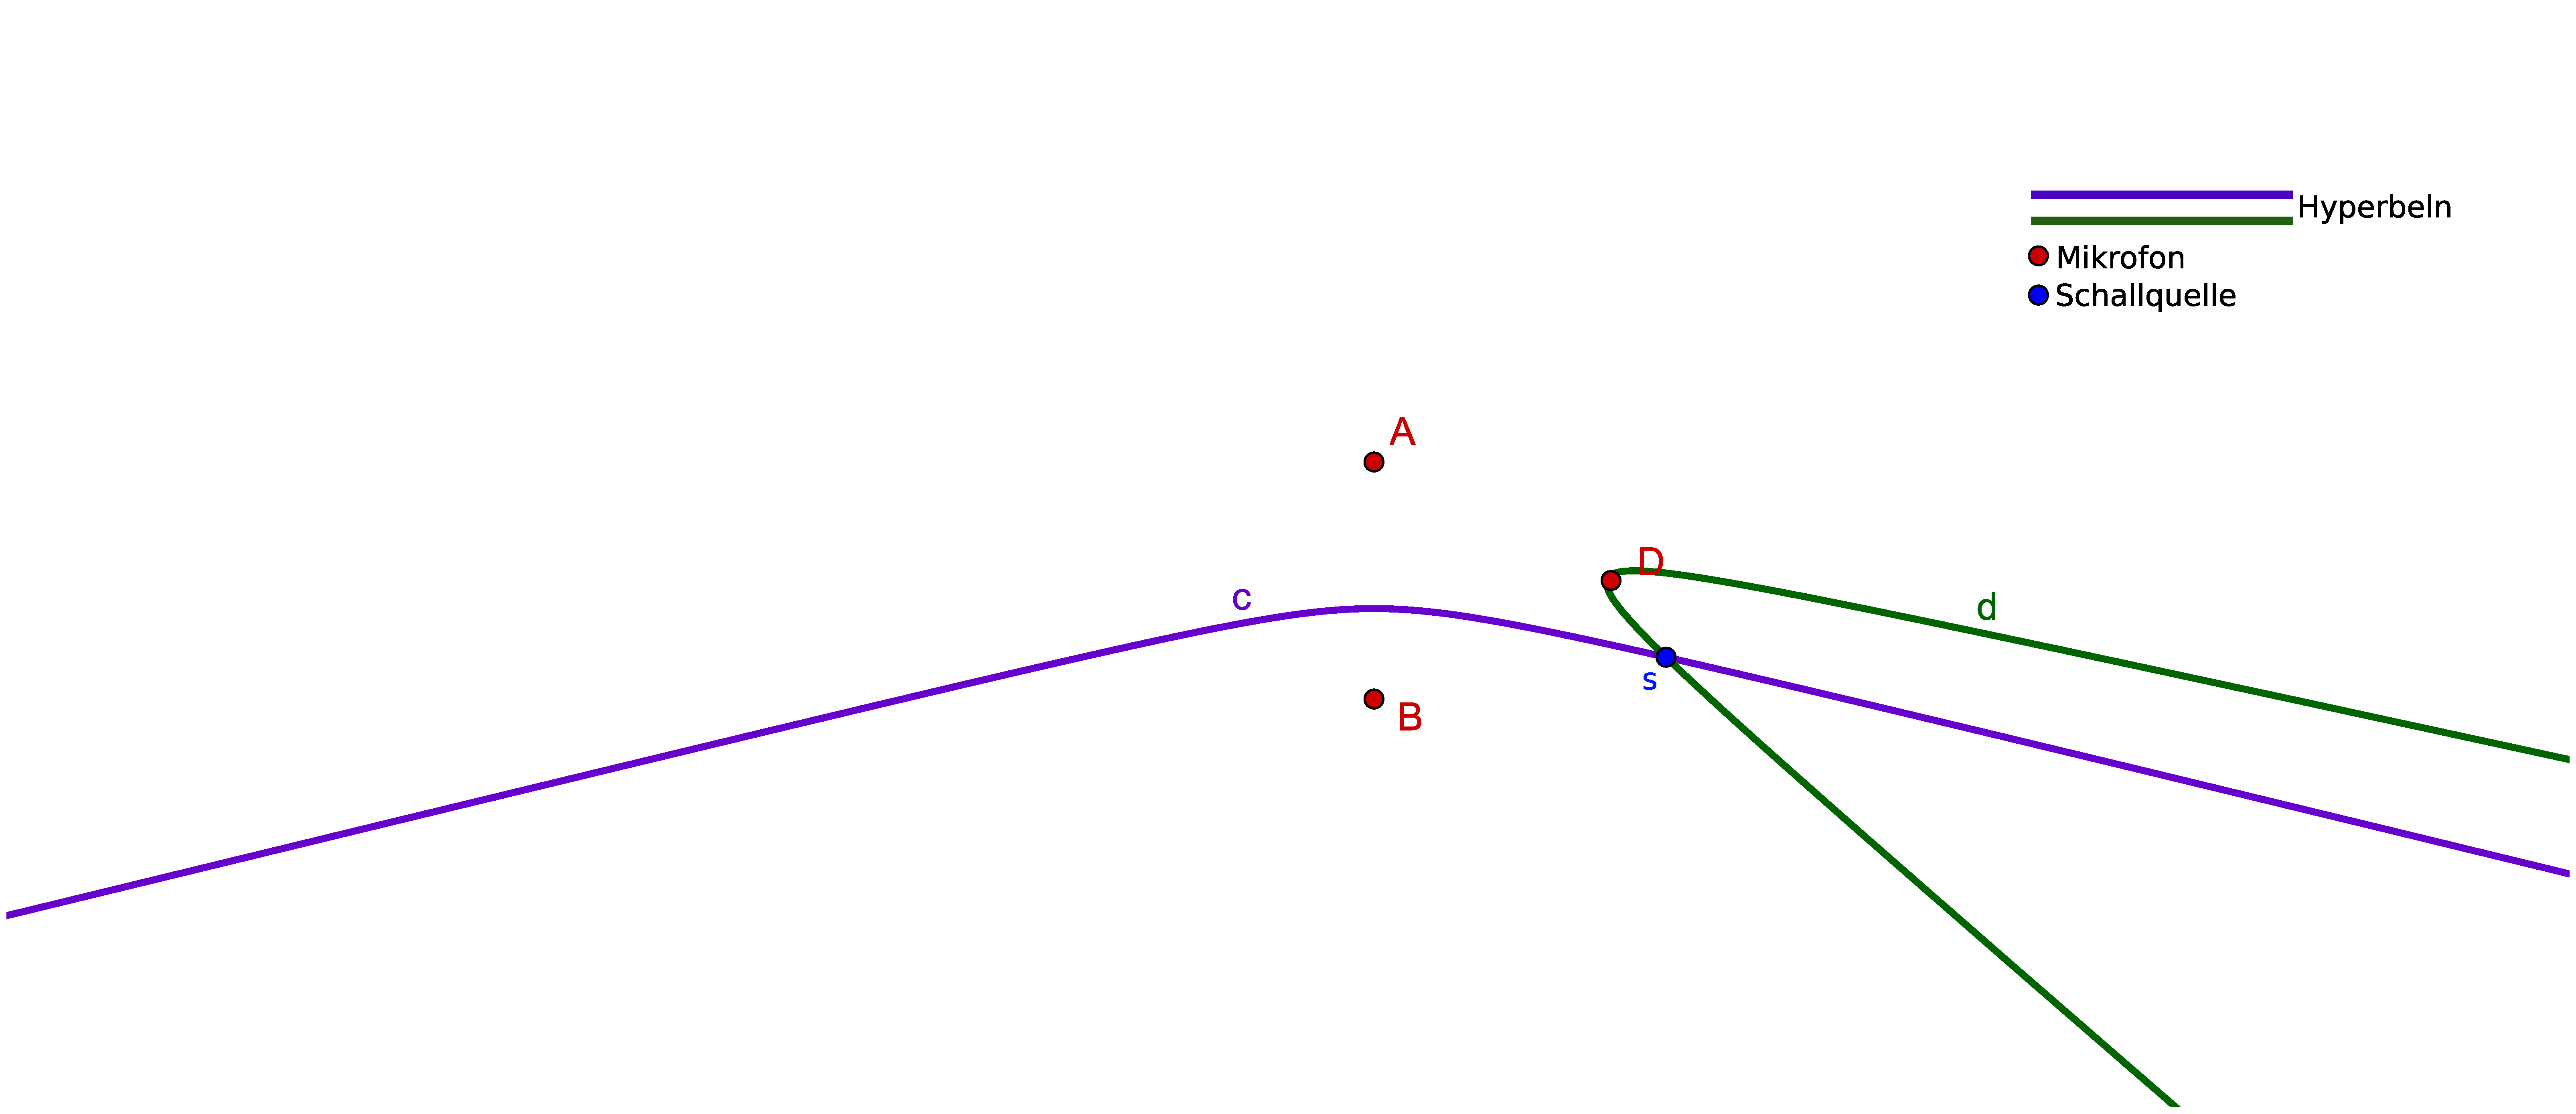
\includegraphics[width=\linewidth]{img/skizze1d}
  \caption{Skizze einer eindimensionalen Richtungsbestimmung}
\label{fig:skizz1d}
\end{figure}

In Abbildung~\ref{fig:skizz1d} sieht man zwei Mikrofone $M_1$ und $M_2$, die den Schall der Schallquelle $S$ aufnehmen. Dadurch, dass $M_2$ weiter von der Schallquelle entfernt ist als $M_1$ braucht der Schall länger um $M_2$ zu erreichen. Wenn man die von den Mikrofonen aufgenommenen Schallwellen vergleicht sieht man dies in Form des rot markierten Gangunterschieds:
\begin{figure}[H]
% GNUPLOT: LaTeX picture with Postscript
\begingroup
  \fontfamily{phv}%
  \selectfont
\definecolor{t}{rgb}{0.5,0.5,0.5}
  \makeatletter
  \providecommand\color[2][]{%
    \GenericError{(gnuplot) \space\space\space\@spaces}{%
      Package color not loaded in conjunction with
      terminal option `colourtext'%
    }{See the gnuplot documentation for explanation.%
    }{Either use 'blacktext' in gnuplot or load the package
      color.sty in LaTeX.}%
    \renewcommand\color[2][]{}%
  }%
  \providecommand\includegraphics[2][]{%
    \GenericError{(gnuplot) \space\space\space\@spaces}{%
      Package graphicx or graphics not loaded%
    }{See the gnuplot documentation for explanation.%
    }{The gnuplot epslatex terminal needs graphicx.sty or graphics.sty.}%
    \renewcommand\includegraphics[2][]{}%
  }%
  \providecommand\rotatebox[2]{#2}%
  \@ifundefined{ifGPcolor}{%
    \newif\ifGPcolor
    \GPcolortrue
  }{}%
  \@ifundefined{ifGPblacktext}{%
    \newif\ifGPblacktext
    \GPblacktextfalse
  }{}%
  % define a \g@addto@macro without @ in the name:
  \let\gplgaddtomacro\g@addto@macro
  % define empty templates for all commands taking text:
  \gdef\gplbacktext{}%
  \gdef\gplfronttext{}%
  \makeatother
  \ifGPblacktext
    % no textcolor at all
    \def\colorrgb#1{}%
    \def\colorgray#1{}%
  \else
    % gray or color?
    \ifGPcolor
      \def\colorrgb#1{\color[rgb]{#1}}%
      \def\colorgray#1{\color[gray]{#1}}%
      \expandafter\def\csname LTw\endcsname{\color{white}}%
      \expandafter\def\csname LTb\endcsname{\color{black}}%
      \expandafter\def\csname LTa\endcsname{\color{black}}%
      \expandafter\def\csname LT0\endcsname{\color[rgb]{1,0,0}}%
      \expandafter\def\csname LT1\endcsname{\color[rgb]{0,1,0}}%
      \expandafter\def\csname LT2\endcsname{\color[rgb]{0,0,1}}%
      \expandafter\def\csname LT3\endcsname{\color[rgb]{1,0,1}}%
      \expandafter\def\csname LT4\endcsname{\color[rgb]{0,1,1}}%
      \expandafter\def\csname LT5\endcsname{\color[rgb]{1,1,0}}%
      \expandafter\def\csname LT6\endcsname{\color[rgb]{0,0,0}}%
      \expandafter\def\csname LT7\endcsname{\color[rgb]{1,0.3,0}}%
      \expandafter\def\csname LT8\endcsname{\color[rgb]{0.5,0.5,0.5}}%
    \else
      % gray
      \def\colorrgb#1{\color{black}}%
      \def\colorgray#1{\color[gray]{#1}}%
      \expandafter\def\csname LTw\endcsname{\color{white}}%
      \expandafter\def\csname LTb\endcsname{\color{black}}%
      \expandafter\def\csname LTa\endcsname{\color{black}}%
      \expandafter\def\csname LT0\endcsname{\color{black}}%
      \expandafter\def\csname LT1\endcsname{\color{black}}%
      \expandafter\def\csname LT2\endcsname{\color{black}}%
      \expandafter\def\csname LT3\endcsname{\color{black}}%
      \expandafter\def\csname LT4\endcsname{\color{black}}%
      \expandafter\def\csname LT5\endcsname{\color{black}}%
      \expandafter\def\csname LT6\endcsname{\color{black}}%
      \expandafter\def\csname LT7\endcsname{\color{black}}%
      \expandafter\def\csname LT8\endcsname{\color{black}}%
    \fi
  \fi
    \setlength{\unitlength}{0.0500bp}%
    \ifx\gptboxheight\undefined%
      \newlength{\gptboxheight}%
      \newlength{\gptboxwidth}%
      \newsavebox{\gptboxtext}%
    \fi%
    \setlength{\fboxrule}{0.5pt}%
    \setlength{\fboxsep}{1pt}%
\begin{picture}(8730.00,3600.00)%
    \gplgaddtomacro\gplbacktext{%
      \colorrgb{0.50,0.50,0.50}%
      \put(990,576){\makebox(0,0)[r]{\strut{}\color{t}$-1$}}%
      \colorrgb{0.50,0.50,0.50}%
      \put(990,857){\makebox(0,0)[r]{\strut{}\color{t}$-0.8$}}%
      \colorrgb{0.50,0.50,0.50}%
      \put(990,1137){\makebox(0,0)[r]{\strut{}\color{t}$-0.6$}}%
      \colorrgb{0.50,0.50,0.50}%
      \put(990,1418){\makebox(0,0)[r]{\strut{}\color{t}$-0.4$}}%
      \colorrgb{0.50,0.50,0.50}%
      \put(990,1699){\makebox(0,0)[r]{\strut{}\color{t}$-0.2$}}%
      \colorrgb{0.50,0.50,0.50}%
      \put(990,1980){\makebox(0,0)[r]{\strut{}\color{t}$0$}}%
      \colorrgb{0.50,0.50,0.50}%
      \put(990,2260){\makebox(0,0)[r]{\strut{}\color{t}$0.2$}}%
      \colorrgb{0.50,0.50,0.50}%
      \put(990,2541){\makebox(0,0)[r]{\strut{}\color{t}$0.4$}}%
      \colorrgb{0.50,0.50,0.50}%
      \put(990,2822){\makebox(0,0)[r]{\strut{}\color{t}$0.6$}}%
      \colorrgb{0.50,0.50,0.50}%
      \put(990,3102){\makebox(0,0)[r]{\strut{}\color{t}$0.8$}}%
      \colorrgb{0.50,0.50,0.50}%
      \put(990,3383){\makebox(0,0)[r]{\strut{}\color{t}$1$}}%
      \colorrgb{0.50,0.50,0.50}%
      \put(1098,396){\makebox(0,0){\strut{}\color{t}$0$}}%
      \colorrgb{0.50,0.50,0.50}%
      \put(1833,396){\makebox(0,0){\strut{}\color{t}$2$}}%
      \colorrgb{0.50,0.50,0.50}%
      \put(2569,396){\makebox(0,0){\strut{}\color{t}$4$}}%
      \colorrgb{0.50,0.50,0.50}%
      \put(3304,396){\makebox(0,0){\strut{}\color{t}$6$}}%
      \colorrgb{0.50,0.50,0.50}%
      \put(4040,396){\makebox(0,0){\strut{}\color{t}$8$}}%
      \colorrgb{0.50,0.50,0.50}%
      \put(4775,396){\makebox(0,0){\strut{}\color{t}$10$}}%
      \colorrgb{0.50,0.50,0.50}%
      \put(5511,396){\makebox(0,0){\strut{}\color{t}$12$}}%
      \colorrgb{0.50,0.50,0.50}%
      \put(6246,396){\makebox(0,0){\strut{}\color{t}$14$}}%
    }%
    \gplgaddtomacro\gplfronttext{%
      \csname LTb\endcsname%
      \put(144,1979){\rotatebox{-270}{\makebox(0,0){\strut{}Amplitude}}}%
      \put(3856,126){\makebox(0,0){\strut{}Zeit[t]}}%
      \csname LTb\endcsname%
      \put(7910,3293){\makebox(0,0)[r]{\strut{}Mikrofon 1}}%
      \csname LTb\endcsname%
      \put(7910,3113){\makebox(0,0)[r]{\strut{}Mikrofon 2}}%
      \csname LTb\endcsname%
      \put(1098,1839){\makebox(0,0)[l]{\strut{}Gangunterschied}}%
    }%
    \gplbacktext
    \put(0,0){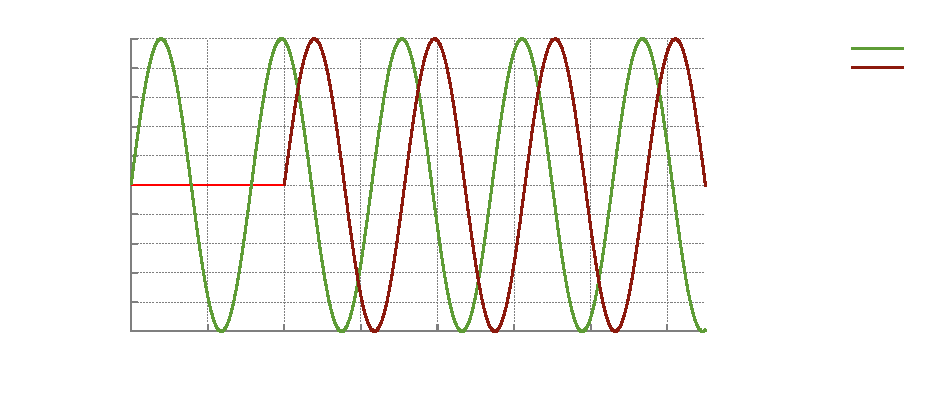
\includegraphics{img/welle1d}}%
    \gplfronttext
  \end{picture}%
\endgroup

\caption{Vergleich der von den beiden Mikrofonen aufgenommenen Wellen}
\label{fig:welle1d}
\end{figure}
Wir können von den von den Mikrofonen aufgenommenen Wellen nur die Phasenverschiebung bestimmen. Deswegen können wir den Gangunterschied nicht direkt bestimmen, er setzt sich aus einer unbekannten Anzahl von kompletten Schwingungen und der Differenz der Phasenverschiebungen zusammen. Man erhält für die Differenz der Abstände einer Schallquelle $S$ von zwei Mikrofonen $M_1$ und $M_2$ mit der gemessenen Phase $\phi_1$ und $\phi_2$: $$n\ + \Delta{x_{12}}$$ $\lambda$ ist hierbei die Wellenlänge, $n$ die unbekannte Anzahl an Schwingungen und $\Delta{x_{12}}$ der Gangunterschied, dem man aus dem Phasenunterschied bestimmen kann:
$$\Delta{x_{ij}} = \frac{c(\phi_i - \phi_j)}{{2\pi}f}\:\textrm{mit}\:i = 1\:\textrm{und}\:j = 2$$
$c$ ist die Schallgeschwindigkeit und $f$ die Frequenz des Schallwelle.
Jedes Mikrofon $M_i$ hat einen zugehörigen Ortsvektor $\vec{m}_i = \begin{pmatrix} m_{i_x} \\ m_{i_y}  \end{pmatrix}$, die Schallquelle hat den Ortsvektor $\vec{s} = \begin{pmatrix} {s_x} \\ {s_y}  \end{pmatrix}$. Der Abstand eines Mikrofons von der Schallquelle ist gegeben durch den Satz des Pythagoras:
$$\abs{\vec{m}_i - \vec{s}} = \sqrt{{(m_{i_x} - s_x)}^2 + {(m_{i_y} - s_y)}^2}$$
Damit erhält man für die Differenz der Abstände der Mikrofone die Gleichung
$$\abs{\vec{m}_1 - \vec{s}} - \abs{\vec{m}_2 - \vec{s}} = n\lambda + \Delta{x_{12}}$$
$$\sqrt{{(m_{1_x} - s_x)}^2 + {(m_{1_y} - s_y)}^2} - \sqrt{{(m_{2_x} - s_x)}^2 + {(m_{2_y} - s_y)}^2} = n\lambda + \Delta{x_{12}}$$$s_y$ ist konstant für alle möglichen Positionen der Schallquelle. Dadurch hat die Gleichung aber immer noch zwei Unbekannte, $s_x$ und $n$, und ist deswegen nicht eindeutig lösbar. Man kann eine eindeutig lösbare Gleichung erhalten, wenn der Abstand der Mikrofone maximal halb so groß wie die Wellenlänge ist. Dann macht die Welle maximal eine halbe Schwingung mehr zu einem Mikrofon als zu dem anderen und die unbekannte Anzahl an Schwingungen $n\lambda$ entfällt. Dann hat die Gleichung nur eine Unbekannte, $s_x$
$$\abs{\vec{m}_1 - \vec{s}} - \abs{\vec{m}_2 - \vec{s}} = \Delta{x_{12}}$$
$$\sqrt{{(m_{1_x} - s_x)}^2 + {(m_{1_y} - s_y)}^2} - \sqrt{{(m_{2_x} - s_x)}^2 + {(m_{2_y} - s_y)}^2} = \Delta{x_{12}}$$
Den dadurch bestimmten Ortvektor kann man dann in eine Gerade $g$ umwandeln, die der Richtung, in der sich die Schallquelle befindet, entspricht:
$$g: \vec{x} = r \cdot \vec{s}$$
Da eine eindimensionale Ortung sehr einfach und ohne großen Anwendungsbereich ist haben wir diesen Algorithmus anschließend auf zwei Dimensionen übertragen.
